\section{Introduction}

\IEEEPARstart{T}{elecommunication}   infrastructures consist of a myriad of technologies from specialized domains such as radio,  access, transport, core and (virtualized) data center networks. Designing, deploying and operating end-to-end services are commonly   manual and long processed performed via traditional \gls{oss} resulting in long lead times (weeks or months) until effective service delivery~\cite{BluePlanet2017ProductsOrchestration}. Moreover, the involved workflows are commonly hampered by built-in hazards of infrastructures strongly coupled to physical topologies and hardware-specific constraints.

Technological advances under the flags of \gls{sdn}~\cite{surveySDN} and \gls{nfv}~\cite{Mijumbi2016NetworkChallenges} bring new ways in which network operators can create, deploy, and manage their services. \gls{sdn} and \gls{nfv} introduce new means for efficient and flexible utilization of their infrastructures through a software-centric service paradigm~\cite{Sonkoly2014UNIFYingView}. However, to realize this paradigm, there is a need to model the end-to-end service and have the ability to abstract and automate the control of physical and virtual resources delivering the service. The coordinated set of activities behind such process is commonly referred to as \textit{orchestration}. In general, orchestration refers to the idea of automatically selecting and controlling multiple resources, services, and systems to meet certain objectives (e.g. a customer requesting a specific network service). Altogether, the process shall be timely, consistent, secure, and lead to cost reduction due to automation and virtualization. 

Multiple stakeholders are involved in the development and standardization of enabling technologies for network softwarization and their embodiment into next generation networks (e.g. 5G) based on \gls{sdn}, \gls{nfv}, and Orchestration building blocks and reference architectures. The ecosystem includes Standards Developing Organizations (SDOs), as well as industry groups, open source projects, foundations, diverse user-lead groups, and so on. Examples of these players include \gls{etsi}, \gls{mef}, \gls{oasis}, Linux Foundation, and \gls{onf}. Similarly, several (academic and industrial) research and (commercial) development efforts in orchestration, SDN and NFV have been going in recent years, concretized in a number of collaborative endeavors such as \gls{osm}~\cite{ETSIOpenMANO}, OpenStack~\cite{Foundationb}, \gls{onap}~\cite{onap}, \gls{5gex}~\cite{Guerzoni2016}, \gls{cord}~\cite{ON.LABOpenCORD},  etc.

Unfortunately,  broad understanding and practical definitions of \gls{nso} are still missing --not only across but also inside networking communities. The maturity of ongoing efforts varies largely with the overall technical approach being very much fragmented and showing little consolidation around an overarching notion of network service orchestration. For instance, the work by Rotsos~et~al.~\cite{Rotsos2017NetworkSurvey} is the first notable attempt to survey the realm of network service orchestration. The authors provide an analysis of the diverse standardization activities around \gls{nso} from an operator perspective. The article follows a top-down approach, defining terminologies, requirements, and objectives of a network service orchestrator. 

\begin{figure*}[th]
  \centering
  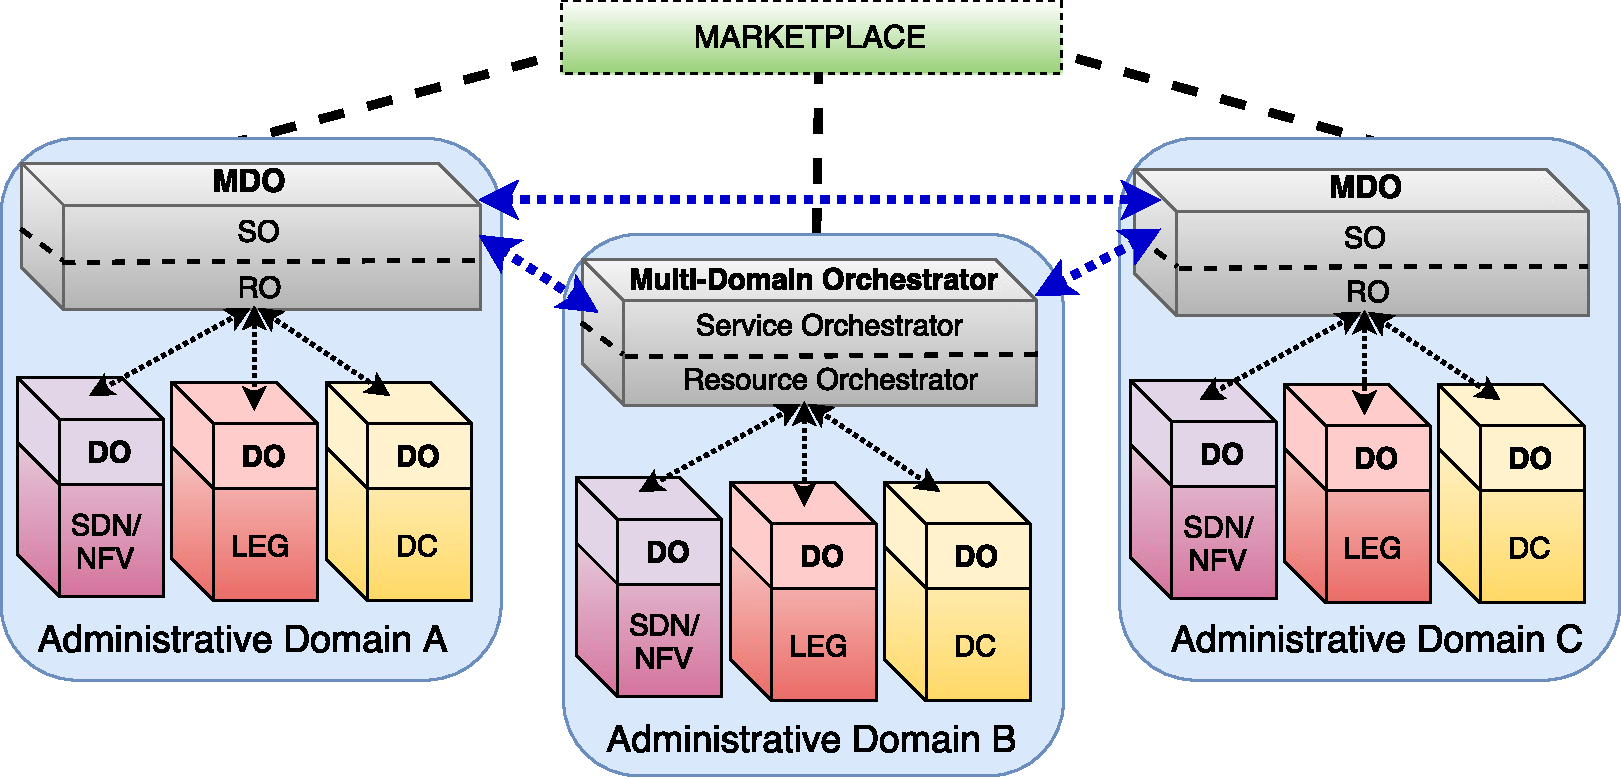
\includegraphics[scale=.6]{Figures/01_Introduction/nso}
    \caption{High-level reference model to illustrate the scope of \acrfull{nso} in single-domain and multi-domain environment. The \gls{nso} need to have an overview of entire environment to compose the service mainly if the service to use resources of different domains.}
    \label{mdo}
\end{figure*}

In this survey, our main objectives are to provide a comprehensive review of research, standardization and software development efforts around the overcharged term of  \acrlong{nso}. We present an in-depth and up-to-date study on network service orchestration covering some history and context, related enabling technologies, standardization activities, actual  solutions, open challenges and  research opportunities. In contrast to~\cite{Rotsos2017NetworkSurvey}, we propose a view of \gls{nso} also from a customer perspective and propose a taxonomy of the main characteristics and features of NSO approaches. We also cover how recent open source platforms and research projects map to the primary characteristics and technical implementations to \gls{nso} realization.    

Throughout the survey, we distinguish between two types of domains. First, \textit{administrative domains}, which map to different organizations and therefore may exist within a single service provider or cover a set of service providers. In one administrative domain, multiple \textit{technology domains} can exist based the type of technology in scope, for example, Cloud, \gls{sdn}, \gls{nfv}, or Legacy. 
Broadly speaking, we refer to \gls{nso} as the automated coordination of resources and services embracing both single-domain and multi-domain contexts.  

Figure~\ref{mdo} presents a generic high-level reference model for multi-domain Network Service Orchestration, featuring  a \gls{mdo} per administrative realm and including the notion of a Marketplace for business interactions. 
\glspl{mdo} coordinate resources and services in a multiple administrative domain scope covering multiple technology domains~\cite{5GPPPArchitectureWorkingGroup2016ViewArchitecture}. 
The exchange of information, resources, and services themselves are essential components of an  end-to-end network service delivery.  The \gls{mdo} exposes the available services to the marketplace allowing service providers to sell network services directly to their customers or other providers under various possible resources consumption models (e.g. trading resources from each other). 
The \gls{mdo} can be seen as a single element with a possible split into two functional components: \gls{so} and \gls{ro}. The \gls{so} orchestrates high-level services while the \gls{ro} is responsible for managing resource and orchestrating workflows  across technology domains. 
The \glspl{do} performs orchestration in each local domain acting on the underlying infrastructures and exposing resources and network functions northbound to the \gls{mdo}. 

\textbf{Survey Organization:} We propose the best of our vision on NSO in this work. The survey is organized as depicted in Figure~\ref{org}. Section~\ref{sec:background} presents essential background and key technologies related to network service orchestration. Concepts, functions, scope, and a taxonomy of NSO are presented in Section~\ref{sec:nso}. Section~\ref{sec:stand} focuses on the standardization efforts whereas Section~\ref{sec:project} covers major research projects around \gls{nso}. Section~\ref{sec:proj} provides an overview of open source and commercial solutions. Section~\ref{sec:scneario} presents some potential scenarios to illustrate the \gls{nso} in practice. The discussion in Section~\ref{sec:challenge} points to a series of open challenges and research opportunities. Finally, Section~\ref{sec:Conclusion} concludes the survey. 
